\documentclass[a4paper]{article}

% Use the postscript times font!
\usepackage{times}
\usepackage{soul}
\usepackage[hyphens]{url}
\usepackage[hidelinks]{hyperref}
\usepackage[utf8]{inputenc}
\usepackage[small]{caption}
\usepackage{graphicx}
\usepackage{amsmath,amssymb}
\usepackage{booktabs}
\usepackage[a4paper, portrait, margin=1in]{geometry}
\urlstyle{same}

\usepackage{parskip}

% the following package is optional:
%\usepackage{latexsym} 

\title{
\includegraphics[scale=0.75]{Resources/unblogo.jpg}\\Application of Artificial Intelligence in Healthcare}

\makeatletter
\renewcommand\@date{{%
  \vspace{-\baselineskip}%
  \large\centering
  \begin{tabular}{@{}c@{}}
    Ethan Garnier\textsuperscript{1} \\
    \normalsize ethan.garnier78@unb.ca 
  \end{tabular}%
  \hspace{3mm}
  \begin{tabular}{@{}c@{}}
    Matthew Tidd\textsuperscript{2} \\
    \normalsize mtidd2@unb.ca
  \end{tabular}
  \hspace{3mm}
  \begin{tabular}{@{}c@{}}
    Minh Nguyen\textsuperscript{2} \\
    \normalsize mnguyen6@unb.ca
  \end{tabular}
  
  \bigskip

  \textsuperscript{1}Department of Electrical and Computer Engineering, UNB\par
  \textsuperscript{2}Department of Mechanical Engineering, UNB

  \bigskip

  \today
}}
\makeatother

\begin{document}

\maketitle

\begin{abstract}
    Artificial intelligence and machine learning are revolutionary tools that enable rapid innovation in many different fields and industries. Healthcare and the medical field are foundational pillars of human society that protect the well-being of people around the world. Recent developments in artificial intelligence and machine learning have shown promise of successfully being applied in the field of medicine to aid physicians and improve quality of care. This paper aims to investigate artificial intelligence's roots in the field of medicine and follow some of its major developments up until today. Some such developments include the use of convolutional neural networks for classifying tumors, machine learning classification of antimicrobial resistance in bacteria, and the early identification of diseases. Due to the nature of artificial intelligence and the stringent regulations surrounding the field of medicine, the implications of applying artificial intelligence in healthcare is also discussed.   
\end{abstract}

\newpage

\section{Introduction}

The world in which we currently live is being transformed by rapid advancements in machine learning and deep learning, heralding the onset of the fourth industrial revolution. Several industries have already leveraged these powerful new technologies and thrust themselves into the forefront of technological advancement, such as in manufacturing \cite{mohd_2022}, agriculture \cite{rashid_2024}, transportation, and governance \cite{qayyum_2021}. As these technologies become more and more entrenched within our daily lives, researchers have begun to turn their attention towards a field once thought impervious to large-scale technological disruptions \cite{qayyum_2021, latif_2017}, the field of healthcare; this field has long been resistant to change due to its high degree of regulation and policy-driven nature. \

Within recent years, the proliferation of advanced algorithms, the advent of widely available Graphics Processing Units (GPUs), and the rapid digitization of patient data and healthcare records have cataylzed a new interest in the development of artificial intelligence for the healthcare industry \cite{jones_2018}. Researchers have developed advanced machine learning tools for the detection and diagnosis of diseases and supportive decision making that enables both healthcare practitioners and patients to enter a new medical ages. \

This paper serves as a survey on the application of artificial intellgience and machine learning in healthcare. To contextualize the development of this technology, this paper first presents an overview of the history of machine learning in medicine within Section 2, recent developments in healthcare artificial intelligence within Section 3, challenges that plague the widespread adoption and implementation of these technologies within Section 4, and each author puts forth a case study within Sections 5-7. Concluding remarks are made within Section 8.\

\section{History of Machine Learning in Medicine}

The medical industry revolves around the collection of data and using that data to make diagnoses to save lives. As such, the application of a tool like machine learning, where learning from data is the focus, is clear in such an industry where data collection is so incredibly important. The history of artificial intelligence and machine learning in medicine spans many decades. Periods of rapid innovation followed by periods of AI "Winters" define this history; however, it begins with the centralization and digitization of medical data that would help propel the research and development of the first prototype medical AI systems.

\subsection{A Medical Library for Machines}

During the beginning of research into AI's potential application in the field of medicine, many issues were raised in regards to how the AI models could be used effectively. The two primary issues were 1) how to connect electronic health records and clinical documentation from around the world, and 2) how can a machine understand the underlying knowledge required for operation in a field as complex and critical as medicine~\cite{kulikowski_beginnings_2019}. Work towards solving these problems began in the 1960's at the National Library of Medicine (NLM), where the Medical Literature Analysis and Retrieval System (MEDLARS), and its web-based search engine, PubMed, would be developed and provide access to the world's largest repository of biomedical literature~\cite{kulikowski_beginnings_2019}. This, alongside the NLM's support of capturing and computationally representing medical terminologies and vocabularies~\cite{kulikowski_beginnings_2019}, essentially solved both of the aforementioned problems. There was now access to the medical data required to train an AI system, and there now existed a computational representation of medical vocabulary and knowledge required for an AI system to confidently operate in the field. It should be noted that the development of these tools was not specifically done for the advancement of AI in medicine; nonetheless, they would prove to be essential in the decades to come.

\subsection{The First AI Winter}

What followed in the 1970's is what many refer to as the first "AI Winter", where there was a significant decrease in interest and investment into the field of AI, not just AI in medicine. Many believe the cause of this first winter to be due to the perceived limitations of artificial intelligence at the time~\cite{kaul_history_2020}, forcing people to disregard the field when in reality it was still in its infancy. Despite this deceleration in research, the 1970's still represented a major stepping stone in the use of AI in medicine. This was accomplished through collaboration between universities across the United States and facilitated by an inter-university time-shared computer system based at Stanford called SUMEX-AIM (Stanford University Medical Experimental - AI in Medicine) developed in 1973~\cite{kulikowski_beginnings_2019}. This collaboration allowed for discussions on many of the concerns that AI's involvement in medicine presented at the time, as well as provided a breeding ground for innovative approaches to the newly developing field. 

\subsection{The First Successful Prototype Systems}

Throughout and following the collaborative innovation of the 1970's was the development of three majorly successful prototype AI systems used for medical diagnosis. These three systems, which will be explained and discussed in this section, provided an idea of what was possible with AI and laid the groundwork for AI's future involvement in the medical field.

\subsubsection{MYCIN}

MYCIN, developed in the 1970's, was a rule-based AI system that used a knowledge-base of roughly 600 rules~\cite{kaul_history_2020} to identify infectious diseases a patient may have and then suggest antibiotic treatment tailored to the patient. Physicians would interface directly with the system by inputting the patient's information and MYCIN would output a list of potential infections, as well as their respective treatments based on information provided about the patient. The list produced by MYCIN was achieved through backward chaining, where MYCIN would start with a given infection and work backwards to try to match it to the patient's symptoms, and used a confidence factor representation to measure clinical uncertainty between the potential diagnoses~\cite{kulikowski_beginnings_2019}. Although this inference method and confidence factor is akin to calculating a probability for a given diagnosis being the correct one, the confidence-factor representation was actually found to psychologically aid in accepting MYCIN consultations~\cite{kulikowski_beginnings_2019}. MYCIN demonstrated that early AI systems had the potential to seriously improve the diagnosis process in medicine, even if only confined to hyper-specific subdomains of the field. Dr. Casimir Kulikowski, one of the authors of CASNET, went on to state that MYCIN "was the most influential expert system that demonstrated the power of modularized rules for representing decision-making"~\cite{kulikowski_beginnings_2019}. The work done on MYCIN and the results it demonstrated would go on to encourage researchers in the field to create more AI prototype systems to aid in diagnosis within different subdomains of medicine, Dr. Kulikowski and his system CASNET being the next one.

\subsubsection{CASNET}

The Causal Associational Network (CASNET) was a consultation program designed specifically for glaucoma patients developed at Rutgers University in the 1970's. CASNET used causal explanations of disease, alongside empirical knowledge of presumptive diagnoses, prognoses, and treatments to advise glaucoma patients~\cite{kulikowski_beginnings_2019}. The CASNET model was divided into three programs~\cite{kaul_history_2020}: model-building, consultation, and a maintained database. By applying disease specific information to a patient of interest, CASNET could provide physicians with patient specific care advice. CASNET was unveiled at the Academy of Ophthalmology meeting in Las Vegas, Nevada in 1976~\cite{kaul_history_2020}.

\subsubsection{INTERNIST-I}

Whereas MYCIN and CASNET were designed to be applied in only small, hyper-specific subdomains of medicine, INTERNIST-I was a system developed to cover a broad range of different medical diagnoses within internal medicine. Developed at the University of Pittsburgh by AI researcher Harry Pople and medicine specialist Dr. Jack Myers~\cite{kulikowski_beginnings_2019}, INTERNIST-I was a prototype AI system designed to assist in general internal medicine diagnosis by modeling the expertise of Dr. Myers~\cite{wolfram_appraisal_1995}. Due to the estimated size of the internal medicine field and the number of diseases it contains, designing a system that could confidently classify symptoms and provide correct diagnoses was a monumental task. Development of INTERNIST-I and its accompanying knowledge-base began in the 1970's, and by 1988 the knowledge-base had grown to contain roughly 600 diseases and represented about 25 person-years of effort~\cite{wolfram_appraisal_1995}. This massive knowledge-base would mean INTERNIST-I would have difficulty with complex diagnosis, when there wasn't a single, clear answer. Despite this drawback, INTERNIST-I would demonstrate that the diagnosis process could be broken down into a pure classification problem, instead of the probabilistic models used by MYCIN and CASNET. As such, INTERNIST-I is considered a crucial step in the development of early AI systems in medicine.

\subsection{The First AI Algorithms}

The advent of AI in medicine provided a training ground to validate the usefulness of the different AI algorithms that had already been established at the time. By observing the impact a training algorithm has in a complicated field such as medicine, researchers would be able to judge how useful the algorithm could be in the greater AI landscape. Focusing only on medical diagnosis at the time of the first AI prototype systems discussed above, there existed two primary AI algorithms being employed: decision trees and Bayesian classification.  

\subsubsection{Decision Trees}
In a medical diagnosis, it is up to the diagnostician to use the patient's symptoms to iteratively rule out possible causes until the final diagnosis is reached. As such, the use of decision trees and decision rules to narrow down a medical diagnosis makes intuitive sense, and early researchers agreed with this. Decision trees were considered to be the most promising area for medical data analysis within a potential AI system~\cite{kononenko_machine_2001}. This promise was further amplified with the invention of the Iterative Dichotomizer 3 (ID3) decision tree algorithm and its application in oncological diagnosis~\cite{kononenko_machine_2001}. Decision trees continued to be a popular option for medical diagnosis due to their more easily interpretable structure. This allowed for the algorithm to better explain its inductive reasoning, re-assuring the physician and the patient on the diagnosis~\cite{kononenko_machine_2001}. 

\subsubsection{Bayesian Classification}
Bayesian classification is a probabilistic approach to inference that uses Bayes' theorem to calculate how likely a given hypothesis is. This naturally maps to the world of medical diagnosis, as given a list of patient symptoms, a Bayesian model assigns probabilities to each potential diagnosis, similar to a physician. Although the transparency, or ability to explain its reasoning through its representation, of Bayesian classification was a cause for concern early on, it was found that using Bayesian classifiers far outperformed other AI algorithms in medical diagnostic tests~\cite{kononenko_machine_2001}. With improvements to the issue of transparency addressed in the 1990's~\cite{kononenko_machine_2001}, Bayesian classification became a commonly used approach in the realm of AI medical diagnosis systems.  

\section{Recent Developments in Healthcare AI}
Ever since the age of big data, there has been a surge in AI developments. 
This acceleration originates from several factors, including the wealth of data collected by big tech, the decreased cost of computational power, developments of more efficient machine learning techniques, and the availability of open-source machine learning packages
The healthcare and medical fields are no exclusion from this wave of AI developments. 
In fact, AI and ML application is an active field of research, receiving attention from researchers, medical stakeholders, and policy makers.
The immersion of the technology in the medical field is evident in the growth of FDA-approved AI/ML-enabled medical devices in \autoref{fig:FDA} \cite{FDA_artificial_nodate}

\begin{figure}[htbp]
    \centering{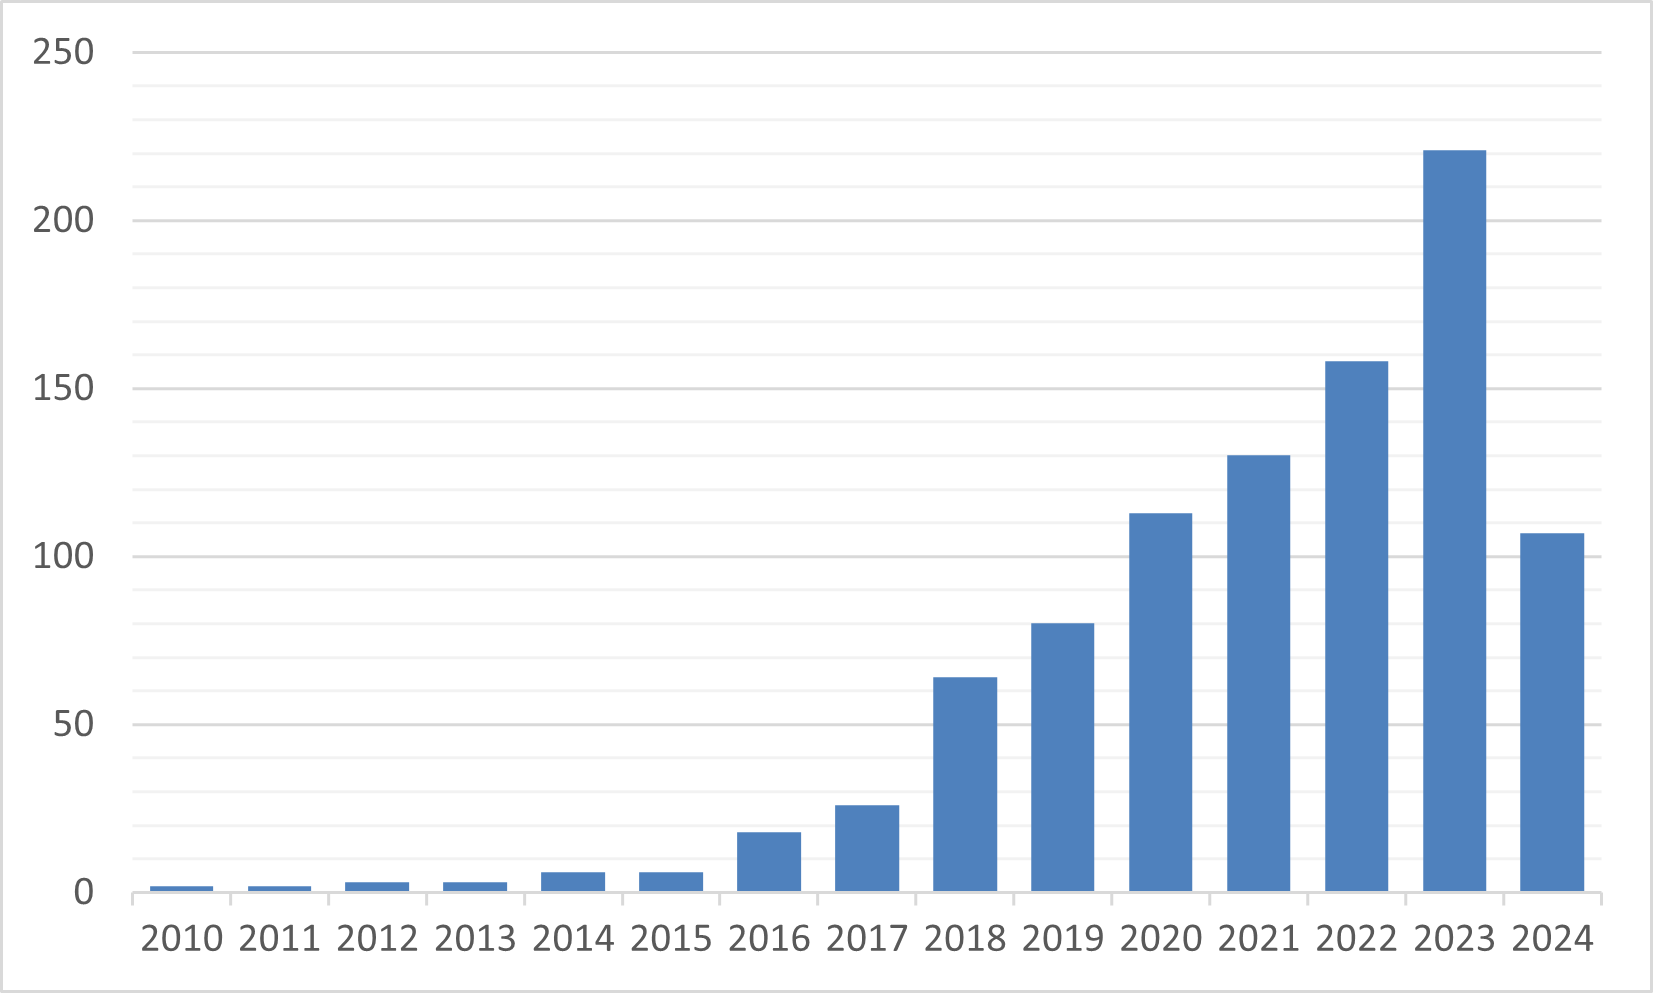
\includegraphics[scale=0.6]{Resources/Growth in ML enabled devices.png}}
    \caption{Number of FDA-approved AI/ML-enabled medical devices since 2010} 
    \label{fig:FDA}
\end{figure}

\subsection{Radiology}
In radiology, machine learning is a powerful tool that can help physisicians with CT scan and MRI scan to diagnose diseases and extract latent insights from the scans. Some example work include
\begin{itemize}
    \item Classification of triple negative breast canser using ultrasound images \cite{wu_machine_2019}
    \item Detection of pulmonary lung nodules from CT scans by convolutional neural network \cite{van_ginneken_off--shelf_2015}
    \item Pneumonia detection from chest X-rays using modern deep learning \cite{rajpurkar_chexnet_2017}
    \item Detection of breast mass from mammography scans using convolutional neural networks \cite{arevalo_convolutional_2015}
\end{itemize} 

\subsection{Dermatology}
In dermatology diagnosis, visual inspection remains the prominent method for determining the severity of a skin abnormalities or lesions. 
Machine learning emerges as an effective automation method as they learn the latent features that differentiate between benign and malignant lesions in skin melanoma. 
As early as 1994, the research in \cite{ercal_neural_1994} applied neural network to automate the classification of malignant melanoma from melanoma-like benign tumors.
The model was given the discriminant characteristics such as tumor shape and relative color, manually extracted from digital images of skin cancer.
In \cite{esteva_dermatologist-level_2017}, a convolutional neural network was trained on 100,000 clinical images of skin cancer and achieved an accuracy similar to that of a dermatologist.
Once these models have been trained extensively on computationally efficient hardware, they can be packaged and deployed on mobile devices to make inferences on skin lesions. 
This can further increase the accessibility of machine learning functionalities to the wider population.


\subsection{Hematology}
In the case of hematological diseases, early prediction can help prevent progression and complication of blood disorders such as leukemia and lymphoma. 
Traditionally, practitioners diagnose hematological conditions by cytomorphologic phenotypic assessment of peripheral blood (PB) and bone marrow (BM) samples.
Newer techniques for disease diagnosis includes flow cytometry and molecular genetic analyses. 
However, diagnostic ambiguity often occurs in such manual process depending on the operator experience and capabilities. 
The reproducibility of clinical results suffer from inter- and intravariations amongst skilled hematologists and pathologists \cite{walter_artificial_2023,wu_hematologist-level_2020}.
Therefore, there needs to be an automated process for reduced reliance on expert knowledge and increased consistency in data interpretation.
Given its predictive power, machine learning implementation in disease diagnosis from blood samples is an active research topic.

In 2014, early developments of automated ML systems for cytomorphologic assessment had limited capabilities, performing tasks such as blood cell counting or classificiation of lymphoid cell types \cite{alomari_automatic_2014,alferez_automatic_2014,alferez_automatic_2015}.
In \cite{guncar_application_2018}, two ML models were developed to predict hematologic disease.
One of them was trained on all available blood test parameters and the other trained on a reduced set of parameters usually obtained from patient admittance.
When this input is paired with the knowledge of the five most likely diseases, the models achieve predictive performance on par with haematology specialists.
In a research by \textit{Wu et al.} \cite{wu_hematologist-level_2020}, the researchers developed a BMSNet with the YOLO-v3 CNN architecture to assist in BM smear interpretation.
The model performance was reported as comparable to that of expert hematologists and pathologists in various tests, except for the classification of myelodysplastic cases.
\textit{Matek et al.} \cite{matek_highly_2021} automated cytomorphologic examination of BM smears by training two CNN-based classifiers. 
The first model has the ResNeXt-50 architecture, previously used in \cite{matek_human-level_2019} for recognition of acute myeloid leukemia blast cells from PB smears due to its low number of hyperparameters.
The second model was a sequential CNN models with a simpler architecture for baseline performance comparison.
The research in \cite{cheuque_efficient_2022} employed a two-stage CNN architecture to classifies four types of white blood cells (leukocytes).
The first layer of CNN leveraged a Faster R-CNN network to delineate the regions of interest and differentiate mononuclear cells from polymorphonuclear cells. 
The seconds layer consists of two parallels CNN with the MobileNet architectures and transfer learning to further categorize the subclasses of leukocytes. 
The lightweight architecture and parallelization in the second layer allows for faster inferencing time.

Flow cytometry or multiparameter flow cytometry (MFC) is a modern techniques for routine blood analysis and an enabling factor for AI integration in hematology.
Modern MPC can analyze thousands of cells a second to generate a large dataset of high dimensional data \cite{walter_artificial_2023}. 
Although this appears challenging for human interpretation and emphasizes the reliance on expert knowledge, a machine learning algorithm can be trained to interpret the latent representation and correlation in the flow cytometry data.
The researchers in \cite{zhao_hematologist-level_2020}, leveraged machine learning by first converting MPC data into multicolor 2D images using a self-organizing map before feeding this data representation through a CNN architecture for classification.
The developed model was capable of categorizing healthy cells from diseased ones, as well as the seven subclasses of mature B-cell neoplasm.

\subsection{Ophthamology}
In the field of ophthamology, a fundoscopy is a non invasive procedure for inestigating the patient's fundus, or the back of their eyes, to diagnose vision conditions and risk factors leading to vision loss.
These detected factors can be used to predict the onset of diseases such as diabetic retinography, glaucoma, retina neoplasms, and macular degeneration \cite{kumar_artificial_2023}

\textbf{Diabetic retinography (DR)} is a condition where high blood sugar level causes damaged vessel in the retina. 
This condition is one of the common causes of vision loss and impairment amongst American living with diabetes and working age adults \cite{commissioner_fda_2020,abramoff_pivotal_2018}.
In 2018, the FDA approved of IDx-DR, the first AI-enabled system for detecting DR.
The research in \cite{abramoff_improved_2016} and \cite{abramoff_pivotal_2018} leveraged a multilayer CNN to train independent detectors for the anatomy and the characteristics of DR, including microaneurysms, hemorhages, and lipoprotein exudates.
The results of these detectors are combined to return the levels of the diseases. 
The study in \cite{sayres_using_2019} implemented an Inception-v4 CNN architecture, to detect the severity grade of DR and provide a heatmap of regions of interest.

Researchers have also integrated AI into the early diagnosis of \textbf{age-related macular degeneration (AMD)}, a chronic and irreversible condition and one of the most common cause of central vision loss. 
One characteristics that signals the onset of AMD is the appearance of hard or soft drusen on optical coherence tomography (OCT) images or color fundoscopy images.
ML can automate the drusen detection to diagnosie early signs of AMD, such as in \textit{Burlina et. al} \cite{burlina_automated_2017} where they employed Deep CNN on color fundus images. The network employs transfer learning on the AlexNet structure, which includes dropout lauers, ReLU activation, and normalization. The weights was trained using stochastic gradient descent and Nesterov momentum, and a learning rate of 0.001 for 50 epochs. This model was compared to a pretrained Overfeat DCNN (New York University) with a linear SVM for classification. The results showed comparable performance to expert human graders, with accuracy ranging from 88.4\% and 91.6\% and an ROC-AUC score betwen 0.94 and 0.96.
In the research done by \textit{Schlegel et al.} \cite{schlegl_fully_2018}, the authors adopted an autoencoder architecture and CNN for learning a simplified representation of the raw images (\autoref{fig:Schlegl_OCT_autoencoder} shows the architecture of this network). The encoder portion of this networks generates an optimized abstract representation of the data embedding, which is then used to re-generate a corresponding image with class labels.
\begin{figure*}[htbp]
    \centering{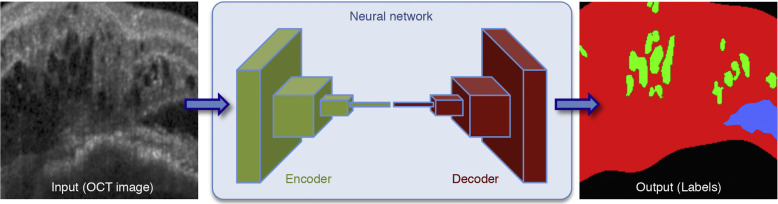
\includegraphics[scale=0.8]{Resources/Schlegl_OCT_autoencoder.jpg}}
    \caption{The proposed network with an autoencoder architecture using CNN in the encoder portion to form a simplified representation of the input features} 
    \label{fig:Schlegl_OCT_autoencoder}
\end{figure*}

\textbf{Glaucoma} is another medical condition resulting in damaged optic nerve. The condition happends when there is a blockage preventing the drainage of the aqueous humor fluid and leading to pressure build-up in the eye.
In \textit{Shibata et al.} \cite{shibata_development_2018}, the authors developed a deep residual network (ResNet) for glaucoma detection from 2D fundus photography. The network is based on the CNN architecture with residual connections to prevent the gradient vanishing and gradient divergence problem, thus allowing for more effective training of deeper networks.
In a recent study by \textit{Thompson et al.} \cite{thompson_assessment_2020}, the authors implemented a deep learning solution for glaucoma detection using B-scan from OCT images. This reseach employed a residual deep convolutional neural network (ResNet34) and transfer learning to leverage the previously trainined feature extraction layers on the ImageNet dataset.

\subsection{Oncology}
The integration of AI and ML systems in cancer treatment is an active branch of research.
Some potential use cases of AI in this field of research are radiotherapy dosage optimization and image segmentation for tissue abnormality detection. AI algorithms have shown promising improvements compared to manual planning in these fields \cite{thompson_artificial_2018}.
In rafiation treament, the prescribed dose is determined by specialist prior to initial treatment. However, the variations in tumour biology poses challenges to this process as the dosage can significantly vary. Further complication may arise depending on the location of the tumour and surrounding organs, thus preventing the desired doseage delivery \cite{huynh_artificial_2020}. In this sense, AI methods can personalize the treatment plan and the optimal prescription achievable depending on the contour of the tumour and organs.
In \textit{Nguyen et al.} \cite{}, the authors leverage the modified U-net CNN network (\autoref{fig:U-Net_architecture_cancer_dose}) to achieve contour-to-dose mapping. Different 

\begin{figure*}[htbp]
    \centering{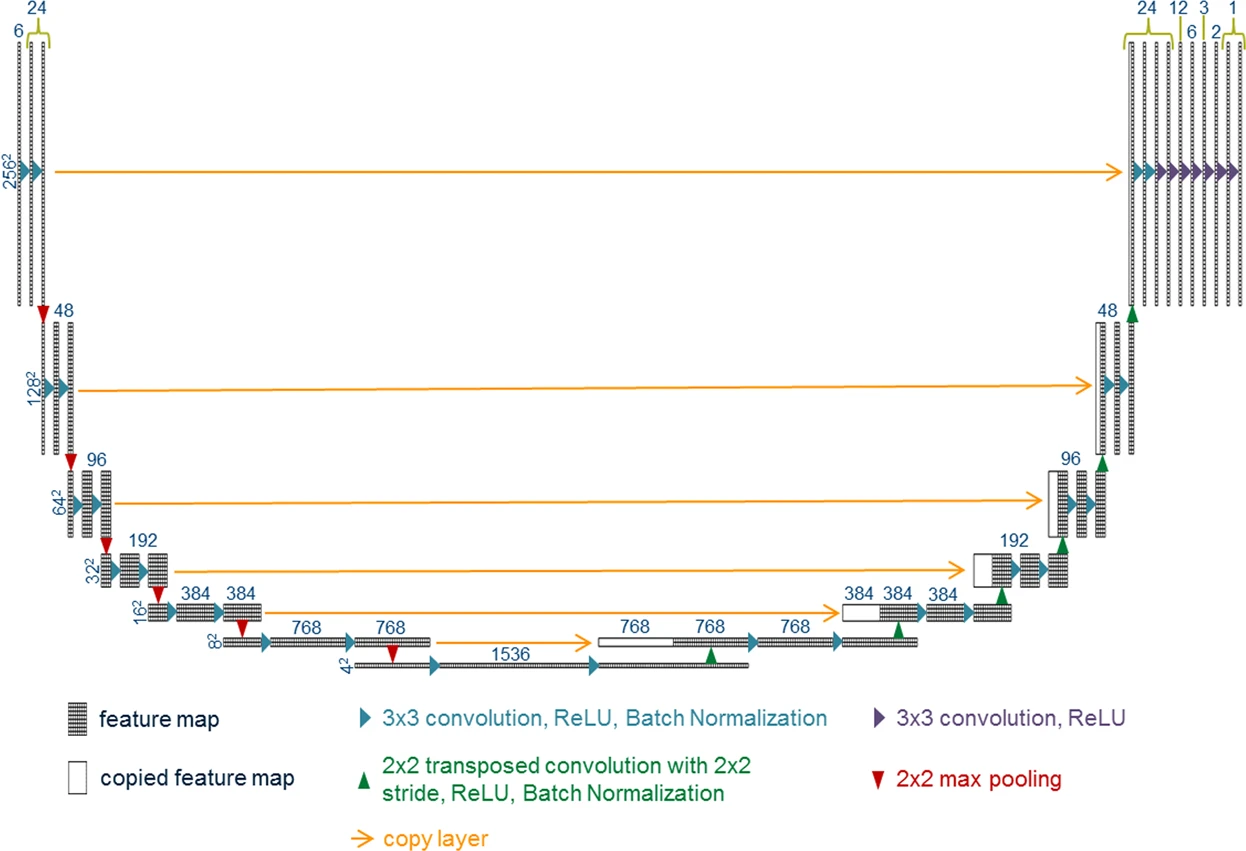
\includegraphics[scale=0.3]{Resources/U-Net CNN Architecture.png}}
    \caption{Modified U-Net architecture for personalized prostate cancer dosage prescription based on patient anatomy}
    \label{fig:U-Net_architecture_cancer_dose}
\end{figure*}

\section{Challenges}

With such an impressive showing of studies wherein machine learning algorithms were leveraged within healthcare for the classification, 
inspection, and detection of several serious radiological, dermatological, haemotological and many other such diseases, it might come across as rather
surprising to learn that real world deployments of machine learning algorithms within clinical practice are rare \cite{Kelly_2019}. There are many reasons for this,
and it is these inherent challenges that plague the widespread adoption and deployment of machine learning algorithms into the field of healthcare as a whole. Within this section
several such key challenges will be highlighted and examined through both an ethical and legalistic lens, as well as pertaining to the disconnect between the design of machine learning algorithms 
and the understanding of those algorithms by medical practitioners. 

\subsection{Adaptation to a Clinical Setting}

As outlined by Kelly et al. in \cite{Kelly_2019}, many challenges arise pertaining to the translation of machine learning models into clinical practice. While many studies have been performed that showcase 
seemingly impressive results within a clinical setting, in reality these studies have been retrospective in nature, that is they have used historically labelled data to train and test algorithms. In reality 
to best understand how these AI systems perform within a true clinical setting, \textit{prospective} studies must be performed. Prospective studies represent the dynamic nature of a clinical setting,
wherein patients are monitored as their medical characteristics or circumstances change as a function of time. In reality, the performance of these AI systems is likely to be worse in prospective studies 
as compared to retrospective studies, as the real-world data collected from a prospective study will vary substantially from the retrospective data used to train the algorithm \cite{Kelly_2019}. 

Another problem that presents itself relates to the nature of machine learning literature. As a common practice within the machine learning community, many studies that are performed are published first to pre-print servers, and not 
to peer-reviewed journals \cite{Kelly_2019}. Due to the stringent nature of the medical community, peer-reviewed evidence will be imperative for the trust and adoption of AI systems within the broader context of the healthcare industry.
The common, so called "gold-standard" of medical research is the use of randomized, controlled trials \cite{Kelly_2019,Khan_2023}, which is not common practice within the machine learning community. As such, high quality reporting of machine learning studies is required for the adoption of these systems into the healthcare industry. For clinicians and medical practitioners to trust and adopt these models into their daily use, there must exist clear and concise reporting on every aspect of these models, such that their usefullness within a clinical setting can be quantified \cite{Kelly_2019}. 

Clinicians and medical practitioners are foremost qualified in medicine, and are not well versed in the knowledge and terminology of machine learning models; as such, many of the metrics that are often utilized within the machine learning community have no tangible meaning to them. As outlined by Kelly et al., "accuracy does not necessarily represent clinical efficacy" \cite{Kelly_2019}. Area under the curve of a receiver operating characteristic curve is a widely used metric within the machine learning community, however it not necessarily the best metric to represent clinicial applicability as it is not easily understandable. 

Similarly, other such metrics such as specificity and sensitivity recorded at a given model operating point, might have no meaning to a doctor who is not well versed in these commonly used terminologies. Arguably the most important factor is that these measure do not reflect what is most important to patients, namely whether the use of the model results in a beneficial change in the care of the patient \cite{Kelly_2019}. Therefore for ML algorithms to be widely adopted within the healthcare industry, these metrics must become more conducive of the clinical understanding of efficacy. Medical students and practicing clinicians should be properly trained in introductory machine learning courses to provide them with the knowledgebase to understand, digest, and adopt these models into their daily workflow.

There are numerous other challenges related to the adoption of machine learning models within a clinical setting. There exists difficulty in comparing models due to the variable methodologies used on datasets with differing distributions. The "dataset-shift" problem also exists, where the introduction of AI models will generate a shift in medical practices, which will cause a change in the dataset used to train these models: effectively chasing a moving target. Current AI models are also far from generalisability, as there exist many unknown variables such as differences in equipment, laboratory equipment, electronic health record systems (EHRs), as well as differences in their codebases. Finally, there exist many logistical difficulties in implementing AI systems, as most healthcare data is not currently stored in a form that is easily digestable by these systems. Data is stored in numerous different mediums, such as medical imaging archival systems, pathology systems, EHRs, insurance databases, and other locations. The amalgamation of all of this data into a single, unifed dataset is a very difficult undertaking \cite{Kelly_2019}. 

When these AI systems make false decisions in automated diagnoses, the results can sometimes be quite harmful to those affected. Due to the nature of EHRs, the data that these machine learning algorithms are trained on is not always the highest quality, or contains numerous inaccuracies. These so called "data errors" can lead to potentially disastrous results, and these "decision errors" have tangible, real effects that affect real patients \cite{Ali_2023}. Similarly, Habehh \& Gohel highlight that the probabilty of error in prediction as well as the impact of this error are downsides of using these models within a clinical setting. Due to how these models rely on probablistic distributions, there is skepticism as to the validity of the predictions made by these models, and the implications of ML-based algorithms failing to operate as intended have severe and potentially fatal repercussions. Finally, they highlight how the rise of ML within the healthcare industry could fuel a decline in the personal relationship that many patients have between the healthcare practitioner, resulting in potential rejection from the public \cite{Habehh_2021}. For these aforementioned reasons, these ML models are far from widespread adaptation into clinical settings, from the perspective of healthcare practitioners and clinicians. 

\subsection{The Black Box Problem}

Another challenge with the use of machine learning algorithms within the healthcare industry is that of the \textit{black box problem}. While this could fall under the section titled Clinical Adaptation, or perhaps the section titled Legal Issues, the author(s) felt it pertinent that this problem recieve its own dedicated section. While the black box problem does factor into why these models are not widely adopted within the healthcare industry from the viewpoint of a clinician, and it also has heavy legal implications, the problem is so inherently intertwined into the inner workings of machine learning that it was given its own section. 

The black box problem relates to the interpretability of a machine learning model, and ones own ability to understand and explain the reasoning as to why and how the output of the model was produced. At its core, this problem stems from how these models are formulated. Large swathes of input data are fed in to train the model to detect patterns that are sometimes anomalous in nature that would be otherwise difficult for a human practitioner to detect. These models then take unforeseen test data and either classify or make a decision based on the type of algorithm. But intrisinic to the functioning of a machine learning algorithm is the manner in which this learning takes place. While we can observe the input and output of the model, we have no way of understanding what is happening within the model itself: this is what is known as the hidden layers. 

These hidden layers learn new representations of the input, and each hidden layer is a re-representation of the input, as information is extracted at higher and higher levels of abstraction. As human operators we have no idea what occurs within the hidden layer. For a deep learning model with millions or even billions of parameters, one can imagine the complexity of the interactions between these parameters and the abstraction that occurs. Therefore the effectiveness of these AI models in the healthcare industry is limited entirely by their own inability to explain their decision making in a way that is understandable \cite{Kelly_2019,Guan_2019}. As one can imagine, this is entirely problematic within the medical industry. A patient is not going to agree to a treatment without first understanding the decision making process that went into determining which treatment was best for them. 

As outlined by Kelly et al., the best performing algorithms are unfortunately the least explainable (deep learning), whereas models with poorer performance are often more explainable (linear regression, decision trees) \cite{Kelly_2019}. If an algorithm ends up making an incorrect decision, or incorrectly recommends something to a healthcare practitioner and they act upon that decision, there is no legal basis for explaining or defending the system as we simply do not know what lead to that decision. This makes it difficult for scientists to understand how data correlates to their predictions, and jeopardizes the faith that the public has in the medical system \cite{Khan_2023}. Therefore the fact that these algorithms cannot be supervised by medical professionals represents a glaring challenge with their implementation and widespread adoption \cite{Murdoch_2021}.

\subsection{Discrimination and Bias}

Another challenge that plagues the implementation of ML into the field of healthcare is that of discrimination and bias. As demonstrated by algorithms implemented into non-medical fields, problematic decisions have been
made by algorithms that reflect biases that are inherently woven into the data used to train them \cite{Char_2018,Khan_2023,Kelly_2019}. These biases stem from systemic problems with the collection of data, such as under-representation of minorities due to racial biases in dataset development, which in turn will lead to subpar prediction results \cite{Khan_2023}. Similarly, 
the implementation of AI systems affect groups that are disadvantaged by factors such as race, gender, and socioeconomic background. Such examples of this within the healthcare industry are mortality prediction algorithms
with accuracy that varies by ethnicity \cite{Chen_2018} and dermatological algorithms that classify both benign and malignant moles with accuracy that could rival a board-certified dermatologist, but with severe underperformance on images of these types of moles when tested on people of colour \cite{esteva_dermatologist-level_2017,Haenssle_2019}.  

The unfairness of an algorithm can be classified into three constituents, such as (1) model bias, where the model elects to best represent the majority but not the under-represented, marginalized groups; (2) model variance, due to inadequate data stemming from minority communities; and (3) outcome noise, such as the effect of unobserved variables that interact with the models predictions \cite{Chen_2018}. 
Algorithms may become biased if there have been no medical studies done in certain populations, and as such the data is lacking \cite{Char_2018}. The result of this is when the algorithm functions as intended, many people benefit. However when the decision making process falters, those that are negatively affected will be from marginalized communities that are under-represented within the very dataset used to train the algorithm, which compounds societal inequities \cite{Panch_2018}.

Price and Cohen outlined bias in action by considering the allocation of scarce medical resources amongst multiple patients. They propose a scenario wherein a particular minority group responds worse off to the proposed medical intervention then other groups, and as such failure to collect information on this minority group would potentially lead to the algorithm giving the minority group more priority than if the data had been included. If the minority group actually responds better to the intervention, the opposite effect could result \cite{price_privacy_2019}.
It is therefore important that strategies to minimize the discrimination of marginalized communities and bias stemming from disparities in datasets between races be implemented throughout the development of machine learning algorithms for use in the healthcare sector.

A bias that was surprising to the author(s) was one that did not stem from the data itself, but rather the intent of those designing the algorithms, as highlighted by Char and Shah in \cite{Char_2018}. They highlight how the medical industry is entering into a new age of privatized development, wherein those responsible for designing ML algorithms for private sector healthcare corporations might be inclined towards malpractice to bolster their algorithm performance. There may exist temptation towards teaching machine learning systems to guide users towards clinical actions that would not necessarily lead to better care, but would lead to better quality metrics and hospital ratings. These systems might be designed in a manner that when they are being scrutinized by health regulators, they skew the data provided for public evaluation. The authors highlight Volkswagen's algorithm for passing emissions test by reducing their nitrogen oxide emissions when tested. Therefore, one must carefully consider the delivate balance between turning a profit and bolstering ratings, and providing improved healthcare for patients. Those responsible for desigining ML for use in healthcare are most likely not healthcare professionals themselves, and therefore need to seriously consider this tension.

\subsection{Data Privacy and Ethics}

Arguably the largest concern with the use of machine learning in the healthcare field is that of data privacy and ethics. As we all know, ML algorithms require copious amounts of data to sufficiently train them to a deployable state. In the context of healthcare, there are often issues with acquiring such a large repository of data. This stems from the fact that patient records are often regarded as confidential, and as such many healthcare organizations are not yet ready to offer up this personable information \cite{Khan_2023}. The deployment of ML systems into the healthcare field has vast implications towards the privacy and confidentiality of data. As early as 1982 some researchers within the medical field were describing the once Hippocratic cornerstone of medicine, confidentiality, as a decrepit and dated concept \cite{Siegler_1982}, an opinion that might be more relevant now than ever.

Char and Shah highlight how the implementation of ML as a decision making support tool into the healthcare field will make confidentiality an increasingly difficult concept to maintain, as patients whose data are not recorded cannot benefit from machine learning analyses \cite{Char_2018}, and the training of ML models will require as much data as possible to ensure clinical accuracy. There also lies the issue in conglomerating health records from all over into one central location, as health records are important and vulnerable data that might be targeted by hackers. There must exist sufficient security measures to prevent data breaches and protect this vulnerable, confidential information \cite{Khan_2023,Ali_2023}. To protect against these kinds of breaches, under the Health Insurance Portability and Accountability Act (HIPAA) patient information is modified by removing a set of 18 specified identifiers, such as names and emails \cite{price_privacy_2019}. Murdoch states in \cite{Murdoch_2021} however that several emerging computational strategies can be used to re-identify individuals in health data breaches, even if the information has been anonymized and scrubbed of identifiers, with success rates as high as 86\% \cite{Murdoch_2021,Check_Hayden_2013,Gymrek_2013,Erlich_2018,Ji_2019}.  

But what if a patient does not want their data to be used to train a ML model? Patient consent therefore becomes a glaring issue, with problems related to informed consent \cite{Gerke_2020,Guan_2019}, consent to data collection \cite{Gerke_2020,Ali_2023,Murdoch_2021}, privacy and consent \cite{Murdoch_2021}, and the extent of consent \cite{Racine_2019,price_privacy_2019} being topics of debate. Informed consent in the context of data management refers to a persons right to know where and how their data is being used, as well as what kinds of data is being used. In terms of data collection, a patient should have consent as to whether or not their information can be used in the training of an ML model. In most recent years, Google has gotten into trouble with their predatory data collection tactics regarding healthcare data being harvested from patients unknowingly.

In 2017 Google's DeepMind partnered with the British NHS Foundation to use machine learning as an assistive tool in the management of acute kidney injury. What users of this app did not know, however, was that their data was inappropriately being annexed from the United Kingdom to the United states, and this private data was collected without the consent or agency of the user \cite{Gerke_2020,Murdoch_2021}. As Murdoch states in \cite{Murdoch_2021}, corporations may not always be encouraged to maintain privacy protection if they can monetize the data or otherwise gain from it, provided that the legal penalties are not high enough to offset this behaviour. In a 2018 survey of four thousand American adults, it was found that only 11\% were willing to share their health data with tech companies, compared to 72\% with physicians. Similarly, only 31\% were either "somewhat confident" or "confident" in the abilities of tech companies to safeguard their data \cite{Murdoch_2021}.

Furthmore, there are concerns about the extent of data collection, and where the line is drawn. Racine et al. highlight that the amount and intrusiveness of health data collection may grow over time as more and more healthcare facilities implement these technologies, highlighting how the development of AI will be used to justify extensive digitization of health status, healthcare practices, treatment use, and even the data collected from wearable devices \cite{Racine_2019}. It is therefore important to consider consent as a dynamic concept, where a patient can track the use of their data and reaffirm their consent if they still wish to. Giving a patient the ability to monitor the evolution of their data as a function of time will allow the patient to have more control over their data, and help to build a trusting relationship between the patient and the healthcare practitioner or ML engineer responsible for the algorithm using their data. Finally, another issue pertaining to consent is whether or not patients should have a role in deciding how their data should be used \cite{price_privacy_2019}, specifically should they be able to decide what gets used from their dataset, and if so, how should it be used?

\section{Case Study: Bias in ML}

In a paper titled \textit{Why Is My Classifier Discriminatory?}, Chen et al. examined the concept of fairness in the context of data, and sought to reduce discriminatory classification by not simply constraining the models used, but rather through augmenting the data collection methodologies used \cite{Chen_2018}. Their paper dealt with automatic decision support systems, like those discussed within this survey. They state that it is often hoped that there will be reduced bias and improved accuracy by training models on observational data, but this is not always the case. Other factors such as data quality and the choice of model however may encode unintentional discrimination, which has a systemically disparate impact \cite{Chen_2018}.

The authors evaluted fairness with respect to protected groups of individuals defined by attributes such as gender and ethnicity, and this paper sought to address the impact of data collection and processign on discrimination and fairness, as this concept was less discussed within the literature compared to constraining the model itself. They describe discrimination in terms of differences in prediciton across all protected groups. In terms of automatic decision support systems, it can often be difficult to balance the tradeoff between predictive accuracy and fairness, as the predictions influence high-states decisions when used in areas such as the healthcare industry \cite{Chen_2018}.

A model was defined as fair if its errors were distributed similarly accross all protected groups, as measured by the cost function $\gamma$. Discrimination was defined as referring to specific kinds of differences in the predictive power of models when applied to these different protected groups. Without diving too deep into the mathematical formulation of their predictive methodology, they based their predictions on a set of covariates:

\begin{center}
    $X \in \chi \subseteq \rm I\!R^k$
\end{center}

\noindent and a \textit{protected attribute}:

\begin{center}
    $A \in \mathcal{A}$
\end{center}

Where $X$ represents the medical history of a patient in critical care, $A$ is the self-reported ethnicity, and $Y$ is mortality. Predictions learned from a training set \textit{d} are denoted as:

\begin{center}
    $\hat{Y}_d := h(X,A)$
\end{center}

Fairness was quantified using a popular cost-based definition known as the equalized odds criterion, which states that a binary classifier \textit{$\hat{Y}$} is fair if its false negative rates (FNR) and false positive rates (FPR) are equal across all groups. FPR and FNR were defined for a member of a protected group $a \in \mathcal{A}$ as:

\begin{center}
    $\text{FPR}_a(\hat{Y}) := \mathbb{E}_X[\hat{Y} \mid Y = 0, A = a], \quad \text{FNR}_a(\hat{Y}) := \mathbb{E}_X[1 - \hat{Y} \mid Y = 1, A = a]$
\end{center}

\noindent The cost function $\gamma$ was defined as:

\begin{center}
    $\gamma_a \in \{\text{FPR}_a, \text{FNR}_a, \text{ZO}_a\}$
\end{center}

Where $\text{ZO}_a$ is the \textit{zero-one loss}, which is a measure of how many mistakes a hypothesis function $h$ makes on the training set, and is given by:

\begin{center}
    $\text{ZO}_a(Y) := \mathbb{E}_X[ \mathbf{1}(Y \neq \hat{Y}) \mid A = a]$
\end{center}

They utilized the MIMIC-III dataset, which is a collection of all clinical notes from 25,879 adult patients from the Beth Israel Deaconess Center, and used this dataset to predict hospital mortality of patients in critical care. Fairness was studied with respect to five self-reported ethnic groups, namely Asian (2.2\%), Black (8.8\%), Hispanic (3.4\%), White (70.8\%), and Other (14.8\%). From the dataset, notes collected in the first 48 hours of an intensive care unit (ICU) stay were used, and patients that stayed for longer than 48 hours were considered. Features were identified by utilizing the tf-idf statistics of the 10,000 most used words from the notes, which assigned a weight to each word based on its frequency relative to the entire document. Their model was trained using 50\% of the data with hyper-parameters selected on 25\%, and tested on 25\%. The model that they used was a logistic regression model with L1-regularization, and they found that it achieved an AUC of 0.81.

Their findings were that Other and Hispanic groups had the highest and lowest generalized zero-one loss, respectively. The largest ethnic group (White) did not have the best accuracy, whereas the smaller ethnic groups tended towards the extremes. Despite having similar base-rates, Black and Hispanic error rates differed drastically. By increasing the training data size by subsampling and splitting the data, holding out at least 20\% for testing, they found that differences in loss decreased with additional training data. Following this, they used clustering to identify clusters where the difference in prediction errors between protected groups was large. This revealed subpopulations for which the differences in zero-one loss were high, which allowed for a more targeted method to reducing discimination. Their work highlights that manipulation of data can be sufficient to improve fairness while maintaining predictive accuracy \cite{Chen_2018}.

\section{Case Study: ML for Antimicrobial Resistance Predictions}

Antimicrobial resistance (AMR) occurs when microbes dangerous to humans and other living creatures evolve and develop resistances to the drugs that are used to combat these microbes. According to the World Health Organization (WHO), AMR and drug-resistant infections are a major threat to global health, with AMR-related deaths projected to reach roughly 10 million by 2050~\cite{balkhy_amr_2021}. As such, AMR is an active area of research as the global health community works to predict, identify, and prevent AMR cases around the world. Innovations in the fields of artificial intelligence (AI) and machine learning (ML) have allowed for their application in the fight against AMR as prediction and decision support systems. This section is a case study on how AI and ML is successfully being applied in the AMR medical field and the results it is yielding.

\subsection{Application of ML in AMR Prediction}

An important step in tackling AMR and drug-resistant infections is identifying resistant pathogens before they have the ability to cause harm. As such, ML is being applied in the classification and identification of potential drug-resistant pathogens through the analysis of their gene contents. The gene contents of available pathogen genomes can be used to predict resistances of those pathogens to various different antibiotics~\cite{kim_machine_2022}. Classification is a common problem solved by AI and ML, hence its usefulness in this area. Training of these predictive models that will be tasked with classifying potentially drug-resistant genomes is accomplished through supervised learning, where genomes that are already labeled as drug-resistant or non-drug-resistant are used to train and test the accuracy of the model. In the context of AMR, there is already an abundance of identified drug-resistant and non-drug-resistant pathogen genomes, as such these pre-labeled genomes are used for training~\cite{kim_machine_2022}.

As with all applications of ML, it is critical that the trained model generalizes well to data it has not seen before. In the context of AMR predictions, this can be a challenge due to several factors surrounding the genomic data sets. First of all, the location, time, and habitat from which samples are taken matters greatly as samples with similar factors can produce large sets of similar genomes, causing a confounding effect in the ML model~\cite{kim_machine_2022}. In addition to this, it is common for genetic data sets to posses an uneven distribution of AMR phenotypes~\cite{kim_machine_2022}, leading to a model incorrectly classifying the majority of examples as the AMR phenotype of majority. Finally, a major difficulty affecting ML model generalization is the potential for poor or contaminated genome assemblies~\cite{kim_machine_2022}. Contaminated data may introduce false positives into the classification process, incorrectly training the model, and resulting in a model that generalizes poorly with non-contaminated data. Given the above reasons, researchers in the field of AMR believe that no single, universal AMR ML model can generalize perfectly and predict drug-resistance in any given pathogen. As such, ML in AMR prediction is being applied in much more specific cases where prediction models are looking to classify genomic data from specific environments or sample cultures as to reduce the confounding effects discussed above~\cite{kim_machine_2022}. I believe that this idea extends past AMR prediction and into the general methodology seen in ML training. Modeling a subset of a given problem is not only easier and far more reasonable, but it can also yield far higher accuracy and potentially provide more utility than a universal solution.

\subsection{ML Algorithms Employed in AMR Prediction}

As was discussed above, AMR prediction is a classification problem in the context of ML. There exists a plethora of classification algorithms commonly used in ML, and many of these have seen application in AMR prediction studies. Gerontini et al~\cite{gerontini_predictions_2011} developed a system to early detect special cases of antibiotic resistance occurring in hospitals through the the use of the Naive Bayes classifier, Support Vector Machines (SVMs), and the C4.5 classification algorithm. This study, which looked to not only solve an AMR related issue but also compare ML classifiers, found that SVMs achieved the best results when compared to the other algorithms according to each test's F-score~\cite{gerontini_predictions_2011}, however this is only in the context of the problem being solved. Sousa et al.~\cite{sousa_validation_2019} employed a decision tree (DT) algorithm to predict a patient's likelihood of infection with a $\beta$-lactamase, an enzyme which renders certain antibiotics inefective, producing organisms. DTs are a very popular classification algorithm employed in the field of AMR prediction, with Goodman et al.~\cite{goodman_predicting_2019} also using DTs to predict the probability of carbapenem-resistant organisms colonization. Y. Kherabi et al.~\cite{kherabi_machine_2024} performed a review of 36 AMR studies where ML models were being applied and found that 42\% of those studies used DTs and 36\% used a derivative of DTs, Random Forests (RF).  

An important factor that impacts the ML classification algorithm chosen is its transparency. As with all ML applications in the field of medicine, ML algorithms applied in the field of AMR must be able to explain their reasoning behind a prediction. Physicians and researchers will not blindly trust the judgment of a model, especially when human health is involved, as such the model's results must be interpretable. Kim et al.~\cite{kim_machine_2022} defines three aspects of interpretability relevant to AMR predictions: ability to evaluate individual input features, traceability, and the ability to assess the interactions of features. The reason why DTs are so popular within this field is due to the fact that they satisfy the above three aspects of interpretability. DTs can rank the important of training features by identifying features that reduce variance~\cite{kim_machine_2022}, and the hierarchical structure of DTs naturally allows for a model's decision path to be traced through each node of the tree. As a result, DTs provide an intuitive explanation to the classification process, making them an excellent algorithm of choice for AMR predictions. 

\subsection{Implications of ML in AMR Prediction}

The threat presented by AMR and drug-resistant infections is a cause for global concern. The advent of AI's application in this fight is a sign of hope; however, this area of research is still in its infancy. The application of AI and ML in clinical decision making causes much ethical concern. When it comes to human life, how can a model be trusted? Although this concern may not be fully understood, it is certainly being respected. In the context of AMR research, ML is being used as a tool to assist in the surveillance and diagnosis of potentially drug-resistant microbes. This often excludes these models from making decisions directly involving patients, and is more of a tool to be used by researchers that will eventually benefit patients down the pipeline. I believe that this is an effective application of ML in the field of medicine as it does not place the responsibility of human life on a ML model, but instead provides an additional tool for experts in the field. In my opinion, in its current form, AI and ML should be used as a tool by the expert, it should not replace the expert. 

\section{Conclusion}


\newpage

% Bibliography/Reference Stuff
\bibliographystyle{ieeetran}
\bibliography{main}
\end{document}